% !TEX root = ../main.tex
% File: chapters_part1/chap2_4.tex
% Nội dung cho Phần 2.4: Mô hình hóa Chủ đề (LDA)

\section{Mô hình hóa Chủ đề (Topic Modeling - LDA)}
\label{sec:topic_modeling_lda}

Cho đến nay, các mô hình chúng ta đã thảo luận chủ yếu thuộc hai loại: học có giám sát (supervised learning) để phân loại hoặc gán nhãn (Naive Bayes, SVM, CRF), hoặc học biểu diễn cho các đơn vị nhỏ như từ (Word2Vec, GloVe). Trong mục cuối cùng của chương này, chúng ta sẽ khám phá một hướng tiếp cận khác hẳn: \textbf{học phi giám sát (unsupervised learning)} để tự động khám phá các \textbf{chủ đề (topics)} tiềm ẩn trong một bộ sưu tập lớn các tài liệu.

Công cụ mạnh mẽ và phổ biến nhất cho nhiệm vụ này là \textbf{Phân bổ Dirichlet Tiềm ẩn (Latent Dirichlet Allocation - LDA)}\cite{blei2003latent}.

\subsection{Tư duy cốt lõi và bài toán}
Hãy tưởng tượng bạn được giao một kho lưu trữ gồm 1 triệu bài báo và được yêu cầu cho biết "Các bài báo này đang nói về những chủ đề chính nào?". Việc đọc thủ công là bất khả thi. Topic Modeling, và cụ thể là LDA, được sinh ra để giải quyết chính xác bài toán này.

LDA được xây dựng dựa trên một loạt các giả định trực quan về cách các tài liệu được "sinh ra":
\begin{enumerate}
    \item Mỗi tài liệu là một \textbf{hỗn hợp của nhiều chủ đề} với các tỷ lệ khác nhau. Ví dụ, một bài báo về việc Apple ra mắt iPhone mới có thể là 70\% chủ đề "Công nghệ", 20\% chủ đề "Kinh doanh" và 10\% chủ đề "Thiết kế".
    \item Mỗi chủ đề là một \textbf{phân phối xác suất trên các từ}. Ví dụ, chủ đề "Công nghệ" sẽ có xác suất cao cho các từ như "máy tính", "phần mềm", "dữ liệu", "AI", và xác suất rất thấp cho các từ như "chính trị", "bầu cử".
\end{enumerate}
Nhiệm vụ của LDA là, khi chỉ được cho xem các tài liệu (tức là các từ), nó phải \textbf{suy ngược (infer)} ra các cấu trúc ẩn đã sinh ra chúng: (1) Hỗn hợp chủ đề cho mỗi tài liệu là gì? và (2) Phân phối từ cho mỗi chủ đề là gì?

\subsection{Câu chuyện sinh dữ liệu của LDA (The Generative Story)}
Cách dễ nhất để hiểu LDA là thông qua "câu chuyện" về cách một tài liệu được tạo ra theo quy tắc của nó. Đây là một thí nghiệm tưởng tượng:

\begin{tcolorbox}[
    title=Câu chuyện sinh dữ liệu,
    colback=orange!5!white, colframe=orange!75!black, fonttitle=\bfseries
]
Giả sử bạn muốn viết một tài liệu mới có $N$ từ, và đã có sẵn một bộ $K$ chủ đề (mỗi chủ đề là một túi từ có xác suất).
\begin{enumerate}
    \item \textbf{Chọn hỗn hợp chủ đề cho tài liệu:} Đầu tiên, bạn quyết định tỷ lệ các chủ đề cho tài liệu của mình. Bạn lấy ngẫu nhiên một vector phân phối chủ đề $\theta_d$ từ một phân phối Dirichlet. Vector này có thể trông như: `[Topic1: 0.7, Topic2: 0.2, Topic3: 0.1, ...]`.
    \item \textbf{Viết từng từ một:} Để viết từ thứ $i$ trong tài liệu (với $i$ từ 1 đến $N$):
        \begin{enumerate}
            \item \textbf{Chọn một chủ đề:} Dựa trên phân phối chủ đề $\theta_d$ của tài liệu, bạn "tung xúc xắc" để chọn ra một chủ đề $z_i$. Ví dụ, với xác suất 70\% bạn sẽ chọn Topic1.
            \item \textbf{Chọn một từ từ chủ đề đó:} Bây giờ bạn đã có chủ đề $z_i$. Mỗi chủ đề lại có một phân phối từ riêng của nó (ký hiệu là $\phi_{z_i}$). Bạn lại "tung xúc xắc" một lần nữa, dựa trên phân phối từ này, để chọn ra một từ $w_i$.
        \end{enumerate}
    \item Lặp lại bước 2 cho đến khi bạn viết đủ $N$ từ.
\end{enumerate}
\end{tcolorbox}

\begin{center}
    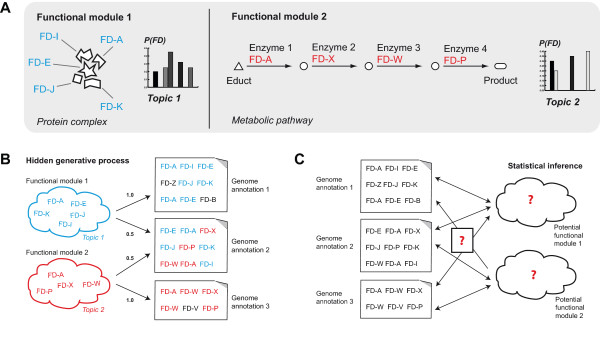
\includegraphics[width=0.9\textwidth]{lda_generative_process.png}
    \captionof{figure}{Mô hình sinh của LDA. Để tạo ra từ $w_{d,n}$ trong tài liệu $d$, mô hình trước hết chọn một chủ đề $z_{d,n}$ từ phân phối chủ đề $\theta_d$ của tài liệu, sau đó chọn từ $w_{d,n}$ từ phân phối từ $\phi_{z_{d,n}}$ của chủ đề đó.}
    \label{fig:lda_generative_process}
\end{center}

Tất nhiên, trong thực tế chúng ta không làm vậy. Chúng ta có sẵn các từ ($w$) và nhiệm vụ của thuật toán LDA là tìm ra các phân phối ẩn $\theta$ (phân phối chủ đề cho mỗi tài liệu) và $\phi$ (phân phối từ cho mỗi chủ đề). Đây là một bài toán suy luận Bayes (Bayesian inference).

\subsection{Huấn luyện và Suy luận trong LDA}
Việc tính toán chính xác các phân phối ẩn trong LDA là bất khả thi về mặt toán học. Do đó, người ta sử dụng các thuật toán xấp xỉ, trong đó phổ biến nhất là \textbf{Lấy mẫu Gibbs (Gibbs Sampling)}.

Trực giác của Lấy mẫu Gibbs như sau:
\begin{enumerate}
    \item \textbf{Khởi tạo:} Đi qua tất cả các từ trong tất cả các tài liệu, gán ngẫu nhiên một trong $K$ chủ đề cho mỗi từ.
    \item \textbf{Lặp lại nhiều lần:} Với mỗi từ $w$ trong một tài liệu $d$:
        \begin{itemize}
            \item Tạm thời "bỏ gán nhãn" chủ đề cho từ $w$.
            \item Tính toán lại xác suất từ $w$ thuộc về mỗi chủ đề $k$, dựa trên hai yếu tố:
                \begin{enumerate}
                    \item Phân phối các chủ đề của các từ khác trong tài liệu $d$ (Tài liệu này đang nói nhiều về chủ đề nào?).
                    \item Phân phối của từ $w$ trên tất cả các tài liệu khác (Từ $w$ này thường xuất hiện trong chủ đề nào?).
                \end{enumerate}
            \item Gán lại một chủ đề mới cho từ $w$ dựa trên xác suất vừa tính được.
        \end{itemize}
\end{enumerate}
Sau khi lặp lại quá trình này rất nhiều lần, việc gán nhãn chủ đề cho các từ sẽ hội tụ về một trạng thái ổn định, phản ánh cấu trúc chủ đề thực sự của kho văn bản. Từ các phân công chủ đề cuối cùng này, chúng ta có thể dễ dàng ước tính $\theta$ và $\phi$.

\subsection{Kết quả và Ứng dụng}
Sau khi huấn luyện một mô hình LDA, chúng ta thu được hai kết quả vô cùng hữu ích:

\paragraph{1. Các chủ đề của kho văn bản}
Mỗi chủ đề được biểu diễn bằng một danh sách các từ có xác suất cao nhất thuộc về nó. Điều này cho phép con người diễn giải ý nghĩa của chủ đề.
\begin{example}{Đầu ra chủ đề của LDA}{ex:lda_topic_output}
    Huấn luyện LDA trên một kho tin tức có thể cho ra các chủ đề như:
    \begin{itemize}
        \item \textbf{Chủ đề 1 (Thể thao):} `bóng đá, đội tuyển, trận đấu, cầu thủ, vô địch, bàn thắng, ...`
        \item \textbf{Chủ đề 2 (Kinh tế):} `cổ phiếu, thị trường, công ty, kinh doanh, tăng trưởng, lạm phát, ...`
        \item \textbf{Chủ đề 3 (Chính trị):} `chính phủ, luật, bầu cử, quốc hội, đảng, quyết định, ...`
    \end{itemize}
\end{example}

\paragraph{2. Biểu diễn tài liệu bằng chủ đề}
Mỗi tài liệu giờ đây có thể được biểu diễn bằng một vector dày đặc, có số chiều bằng số chủ đề $K$. Mỗi chiều của vector là tỷ lệ của chủ đề đó trong tài liệu.
\begin{example}{Biểu diễn tài liệu bằng LDA}{ex:lda_doc_representation}
    Một bài báo có nội dung "Đội tuyển bóng đá quốc gia giành chức vô địch sau một trận đấu kịch tính" có thể được biểu diễn bằng vector:
    `[Thể thao: 0.9, Kinh tế: 0.05, Chính trị: 0.05]`
\end{example}

\textbf{Ứng dụng thực tế của LDA:}
\begin{itemize}
    \item \textbf{Khám phá dữ liệu:} Nhanh chóng nắm bắt các chủ đề chính trong một kho văn bản lớn.
    \item \textbf{Hệ thống gợi ý (Recommender Systems):} Gợi ý các bài báo tương tự cho người dùng dựa trên sự tương đồng về phân phối chủ đề.
    \item \textbf{Kỹ thuật đặc trưng (Feature Engineering):} Sử dụng các vector chủ đề làm đặc trưng đầu vào cho các mô hình phân loại có giám sát. Thay vì dùng một vector BoW hàng chục ngàn chiều, chúng ta có thể dùng một vector chủ đề chỉ vài trăm chiều, vừa giảm chiều dữ liệu vừa mang tính ngữ nghĩa cao.
\end{itemize}

\subsection{Ưu và Nhược điểm}
\begin{tcolorbox}[
    title=Đánh giá mô hình LDA,
    colback=blue!5!white, colframe=blue!50!black, fonttitle=\bfseries
]
\textbf{Ưu điểm:}
\begin{itemize}
    \item \textbf{Học phi giám sát:} Không cần dữ liệu gán nhãn, cực kỳ hữu ích cho việc khám phá.
    \item \textbf{Cung cấp kết quả diễn giải được:} Con người có thể đọc và hiểu ý nghĩa của các chủ đề.
    \item \textbf{Là một kỹ thuật giảm chiều dữ liệu mạnh mẽ.}
\end{itemize}
\textbf{Nhược điểm:}
\begin{itemize}
    \item \textbf{Phải chọn trước số chủ đề ($K$):} Việc chọn giá trị $K$ tối ưu là một thách thức và thường đòi hỏi thử nghiệm.
    \item \textbf{Giả định Bag-of-Words:} LDA bỏ qua trật tự từ, giống như BoW.
    \item \textbf{Các chủ đề có thể không mạch lạc:} Đôi khi mô hình tạo ra các chủ đề là một mớ hỗn độn các từ có tần suất cao nhưng không có ý nghĩa rõ ràng.
\end{itemize}
\end{tcolorbox}

\bigskip
\hrule
\bigskip

\begin{center}
    \textbf{\Large KẾT THÚC CHƯƠNG 2}
\end{center}

\textit{Chương 2 đã đưa chúng ta vào một hành trình qua kỷ nguyên thống kê, từ việc biểu diễn văn bản như những "túi từ" đơn giản đến các vector ngữ nghĩa phức tạp. Cuộc cách mạng Word Embeddings đã cho chúng ta thấy rằng ý nghĩa của từ có thể được nắm bắt trong các không gian vector dày đặc, một ý tưởng nền tảng cho toàn bộ NLP hiện đại. Tuy nhiên, các embedding tĩnh này vẫn chưa nắm bắt được sự thay đổi của ý nghĩa theo ngữ cảnh. Đây chính là động lực để chúng ta bước sang chương tiếp theo, khám phá các kiến trúc mạng nơ-ron được thiết kế để "đọc" và "ghi nhớ" các chuỗi văn bản, mở ra kỷ nguyên của sự hiểu biết ngữ cảnh sâu sắc.}